\documentclass{standalone}
\usepackage{tikz}
\usetikzlibrary{calc}

\begin{document}
	
	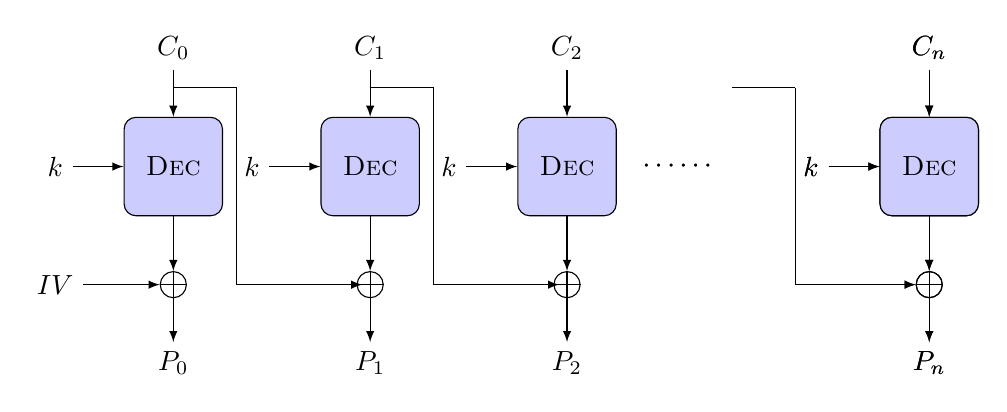
\begin{tikzpicture}
		
		\foreach \x in {0, 1, 2} {
			\node (f\x) at ($\x*(2.5cm,0)$) [minimum size=1.25cm,rounded corners=1ex,fill=blue!20,draw] {{\sc Dec}};
			\node (c\x) [below of=f\x, node distance=2.5cm] {$P_\x$};
			\node (k\x) [left of=f\x, node distance=1.5cm] {$k$};
			\node (p\x) [below of=f\x, node distance=1.5cm, circle, draw] {};
			\node (m\x) [above of=f\x, node distance=1.5cm] {$C_\x$};
			\draw[-] (p\x.north) -- (p\x.south);
			\draw[-] (p\x.east) -- (p\x.west);
			\draw[-latex] (m\x) -- (f\x);
			\draw[-latex] (f\x) -- (p\x);
			\draw[-latex] (k\x) -- (f\x);
			\draw[-latex] (p\x) -- (c\x);
		}
		
		\node (iv) [left of=p0, node distance=1.5cm] {$IV$};
		\draw[-latex] (iv) -- (p0);
		
		\foreach \x in {0, 1} {
			\draw[-latex] ($(m\x) - (0,0.5cm)$) -| +(0.8cm,-2.5cm) -- ($(p\x) + (2.4cm,0)$);
			
			\begin{scope}
				\node at (6.4,0) {$\cdots\cdots$};
			\end{scope}
			
			\begin{scope}
				\node (f) at (9.6cm,0) [minimum size=1.25cm,rounded corners=1ex,fill=blue!20,draw] {{\sc Dec}};
				\node (c) [below of=f, node distance=2.5cm] {$P_n$};
				\node (k) [left of=f, node distance=1.5cm] {$k$};
				\node (p) [below of=f, node distance=1.5cm, circle, draw] {};
				\node (m) [above of=f, node distance=1.5cm] {$C_n$};
				\draw[-] (p.north) -- (p.south);
				\draw[-] (p.east) -- (p.west);
				\draw[-latex] (m) -- (f);
				\draw[-latex] (f) -- (p);
				\draw[-latex] (k) -- (f);
				\draw[-latex] (p) -- (c);
				\draw[-] ($(m) - (2.5,0.5cm)$) -- ($(m) - (1.7,0.5cm)$);
				\draw[-latex] ($(m) - (1.7,0.5cm)$) |- + (0cm,-2.5cm) -- (p);
			\end{scope}
		}
		
	\end{tikzpicture}
	
\end{document}